\chapter{Subdomain Neumann-Ulam Scaling with Multiple Sets\ }
\label{chap:extra_scaling}
As an additional analysis of MCSA using subdomain Monte Carlo, the multiple
sets scaling studies are repeated to determine if any performance
benefits are made from replication by eliminating Monte Carlo
communication. Figure~\ref{fig:titan_strong_subdomain_ms_time} gives
the runtimes for the strong scaling calculation and
Figure~\ref{fig:titan_strong_subdomain_ms} the computed absolute
efficiencies. For the weak scaling studies,
Figure~\ref{fig:titan_weak_subdomain_ms_time} gives the wall times and
Figure~\ref{fig:titan_weak_subdomain_ms} the efficiencies. For both
scaling studies, the results are effectively the same as for the case
with Monte Carlo communication. This is again due to the fact that
adding sets to the problem is not only an exercise in strong scaling
but it also adds additional parallel overhead in the form of the tally
vector reduction across blocks.

\begin{figure}[t!]
  \begin{center}
    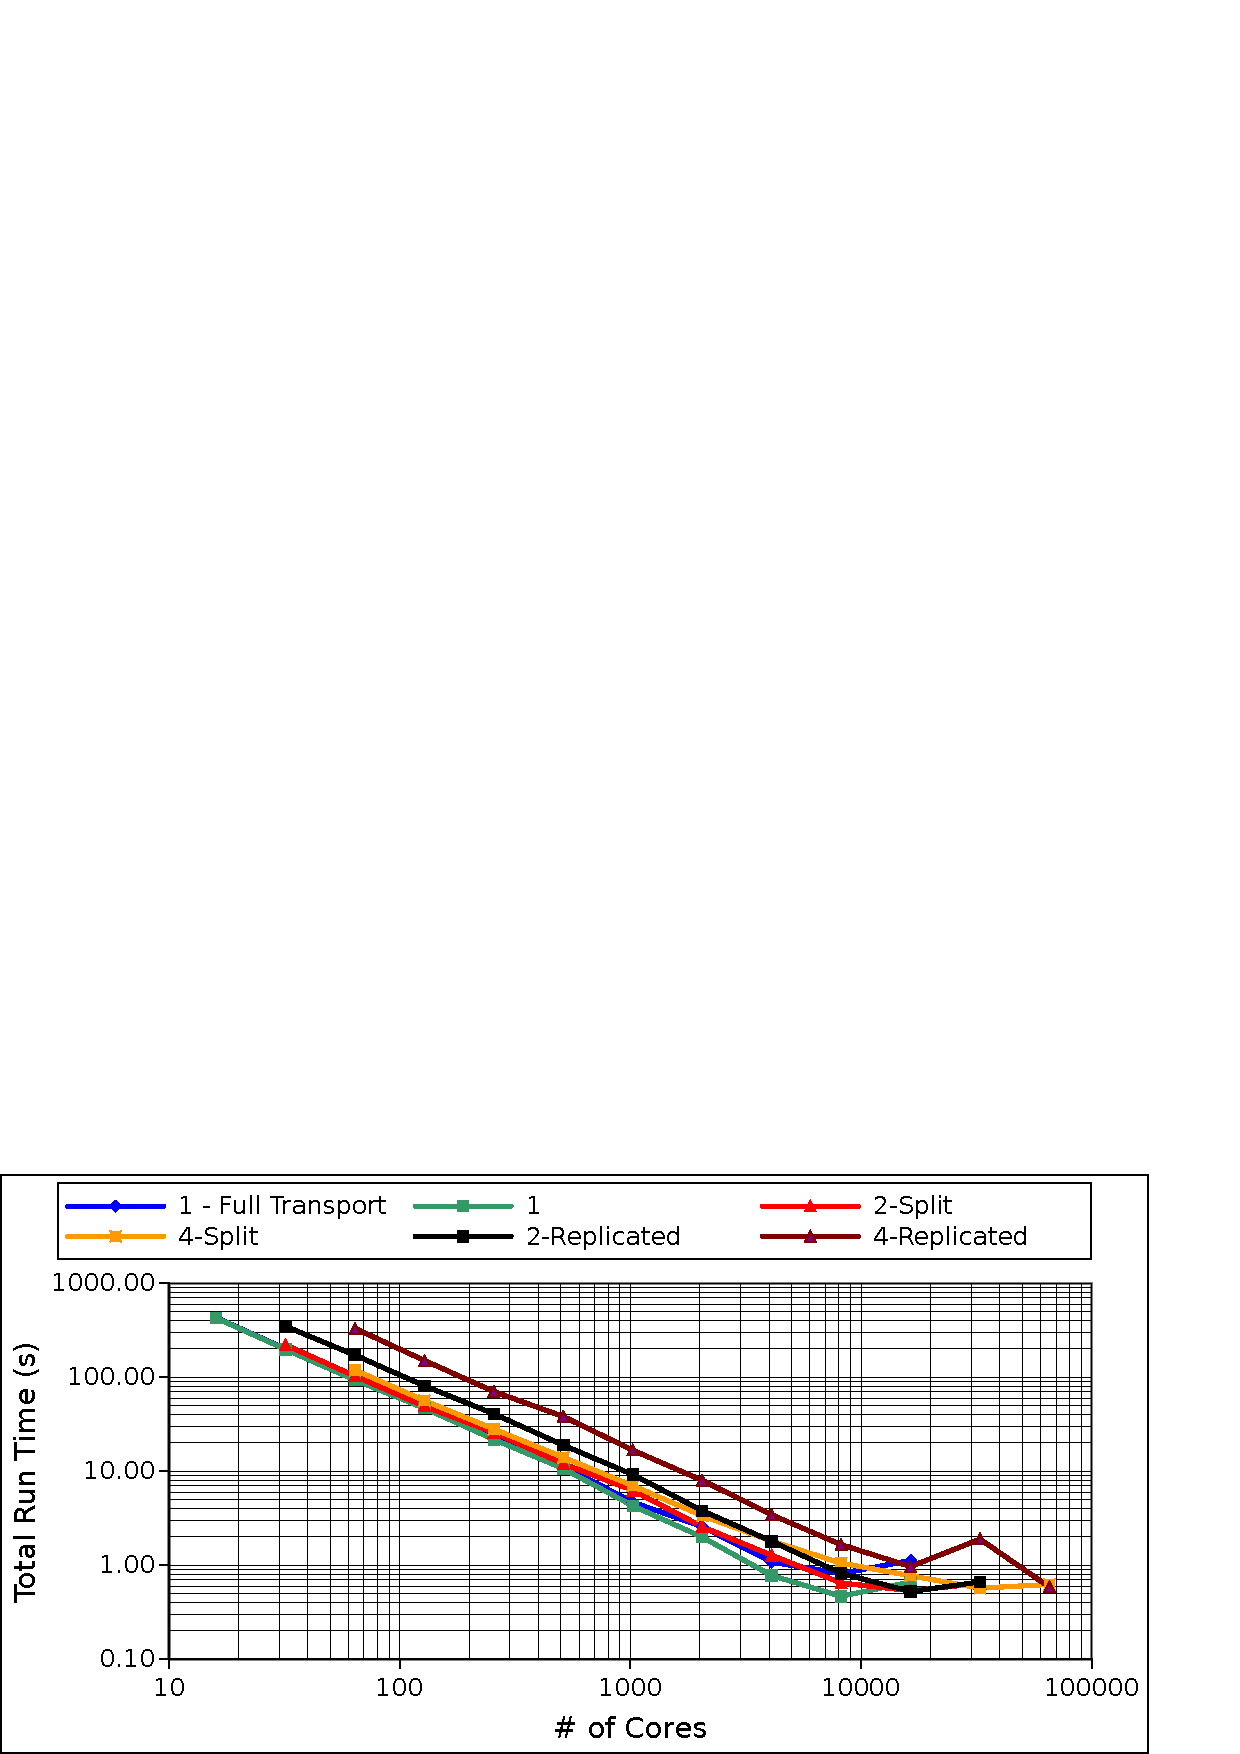
\includegraphics[width=6in]{chapters/parallel_mc/titan_strong_subdomain_ms_time.pdf}
  \end{center}
  \caption{\textbf{Strong scaling total wall time with multiple sets
      and subdomain Monte Carlo.} \textit{Adding multiple sets has in
      general a negative effect on the wall time as was observed for
      the case with full Monte Carlo transport.}}
  \label{fig:titan_strong_subdomain_ms_time}
\end{figure}

\begin{figure}[t!]
  \begin{center}
    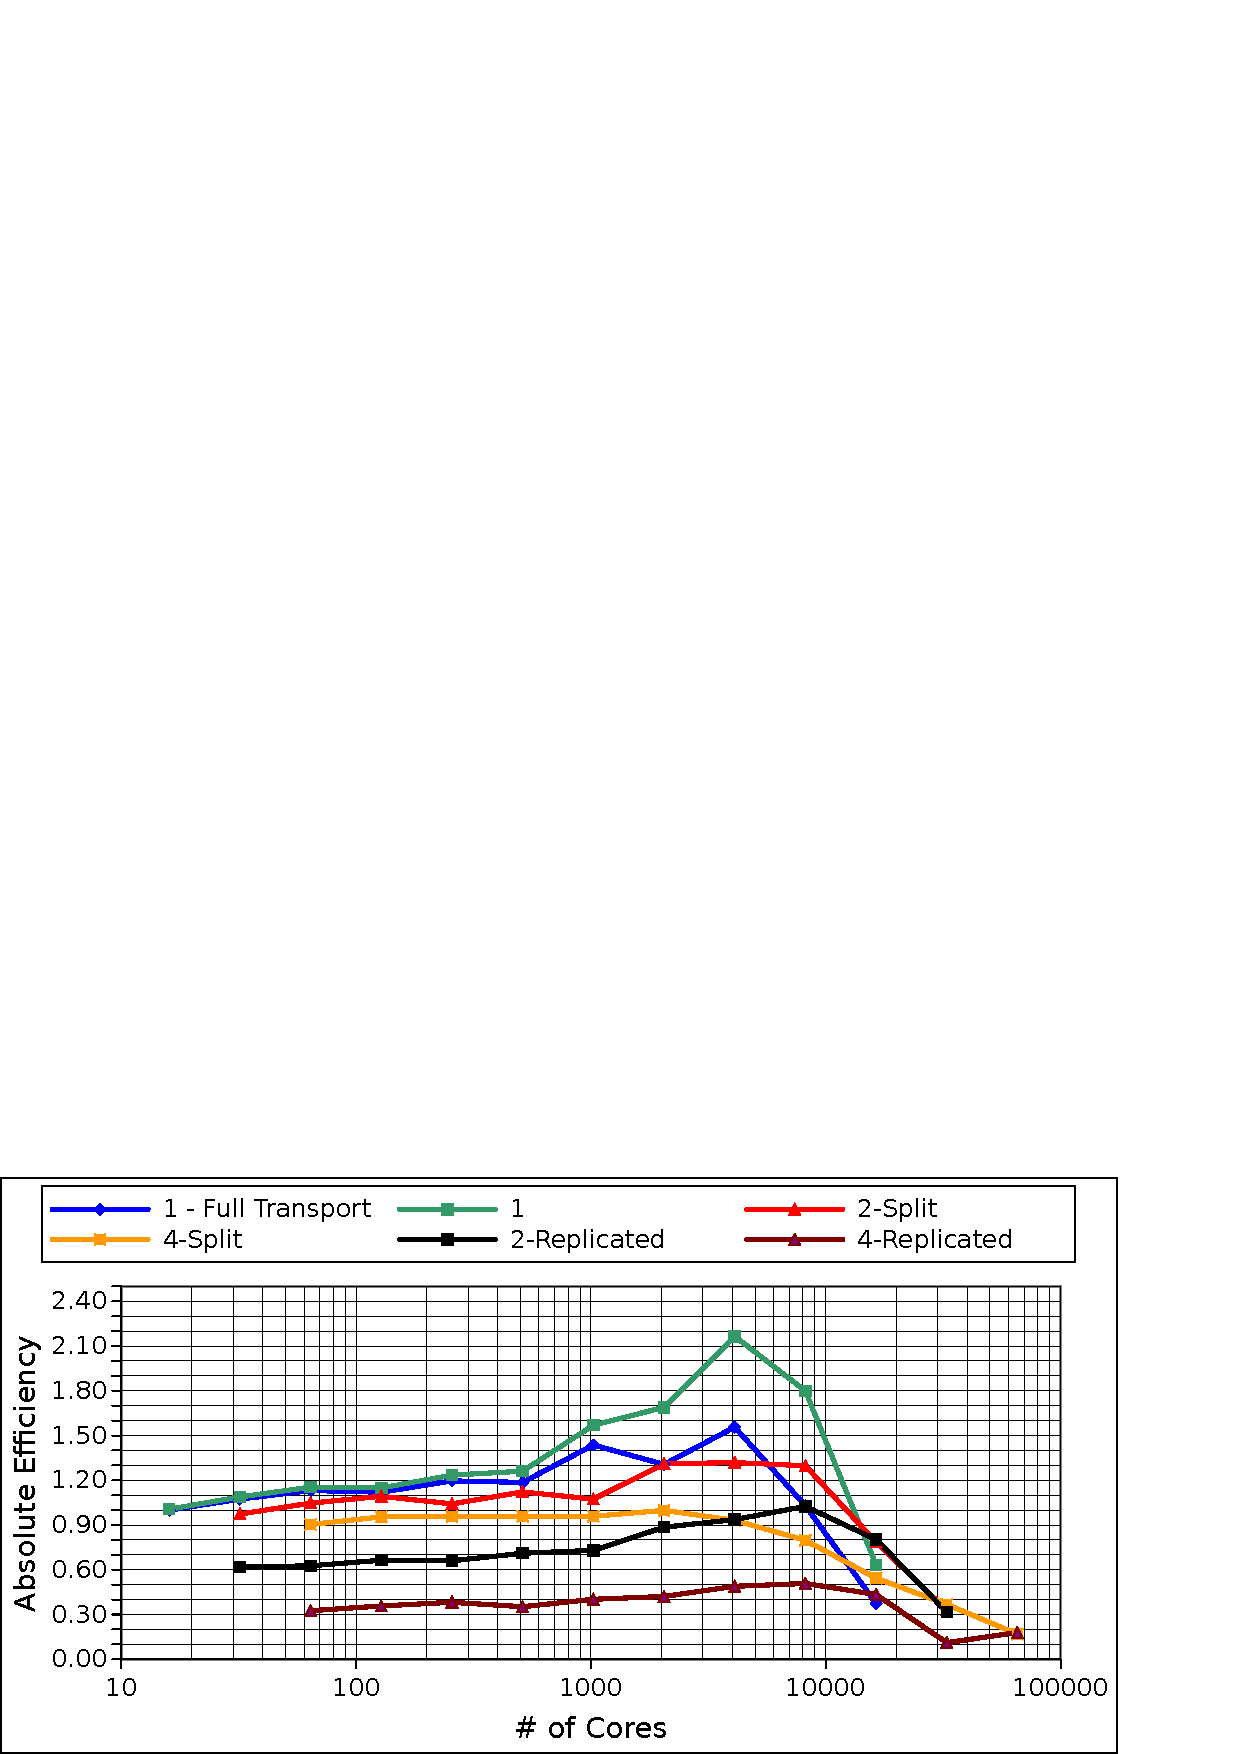
\includegraphics[width=6in]{chapters/parallel_mc/titan_strong_subdomain_ms.pdf}
  \end{center}
  \caption{\textbf{Strong scaling absolute efficiency for with
      multiple sets and subdomain Monte Carlo.} \textit{Increased wall
      times from adding parallel reduction operations for multiple
      sets reduces parallel scalability at lower core counts but gives
      a higher efficiency at the strong scaling wall.}}
  \label{fig:titan_strong_subdomain_ms}
\end{figure}

\begin{figure}[t!]
  \begin{center}
    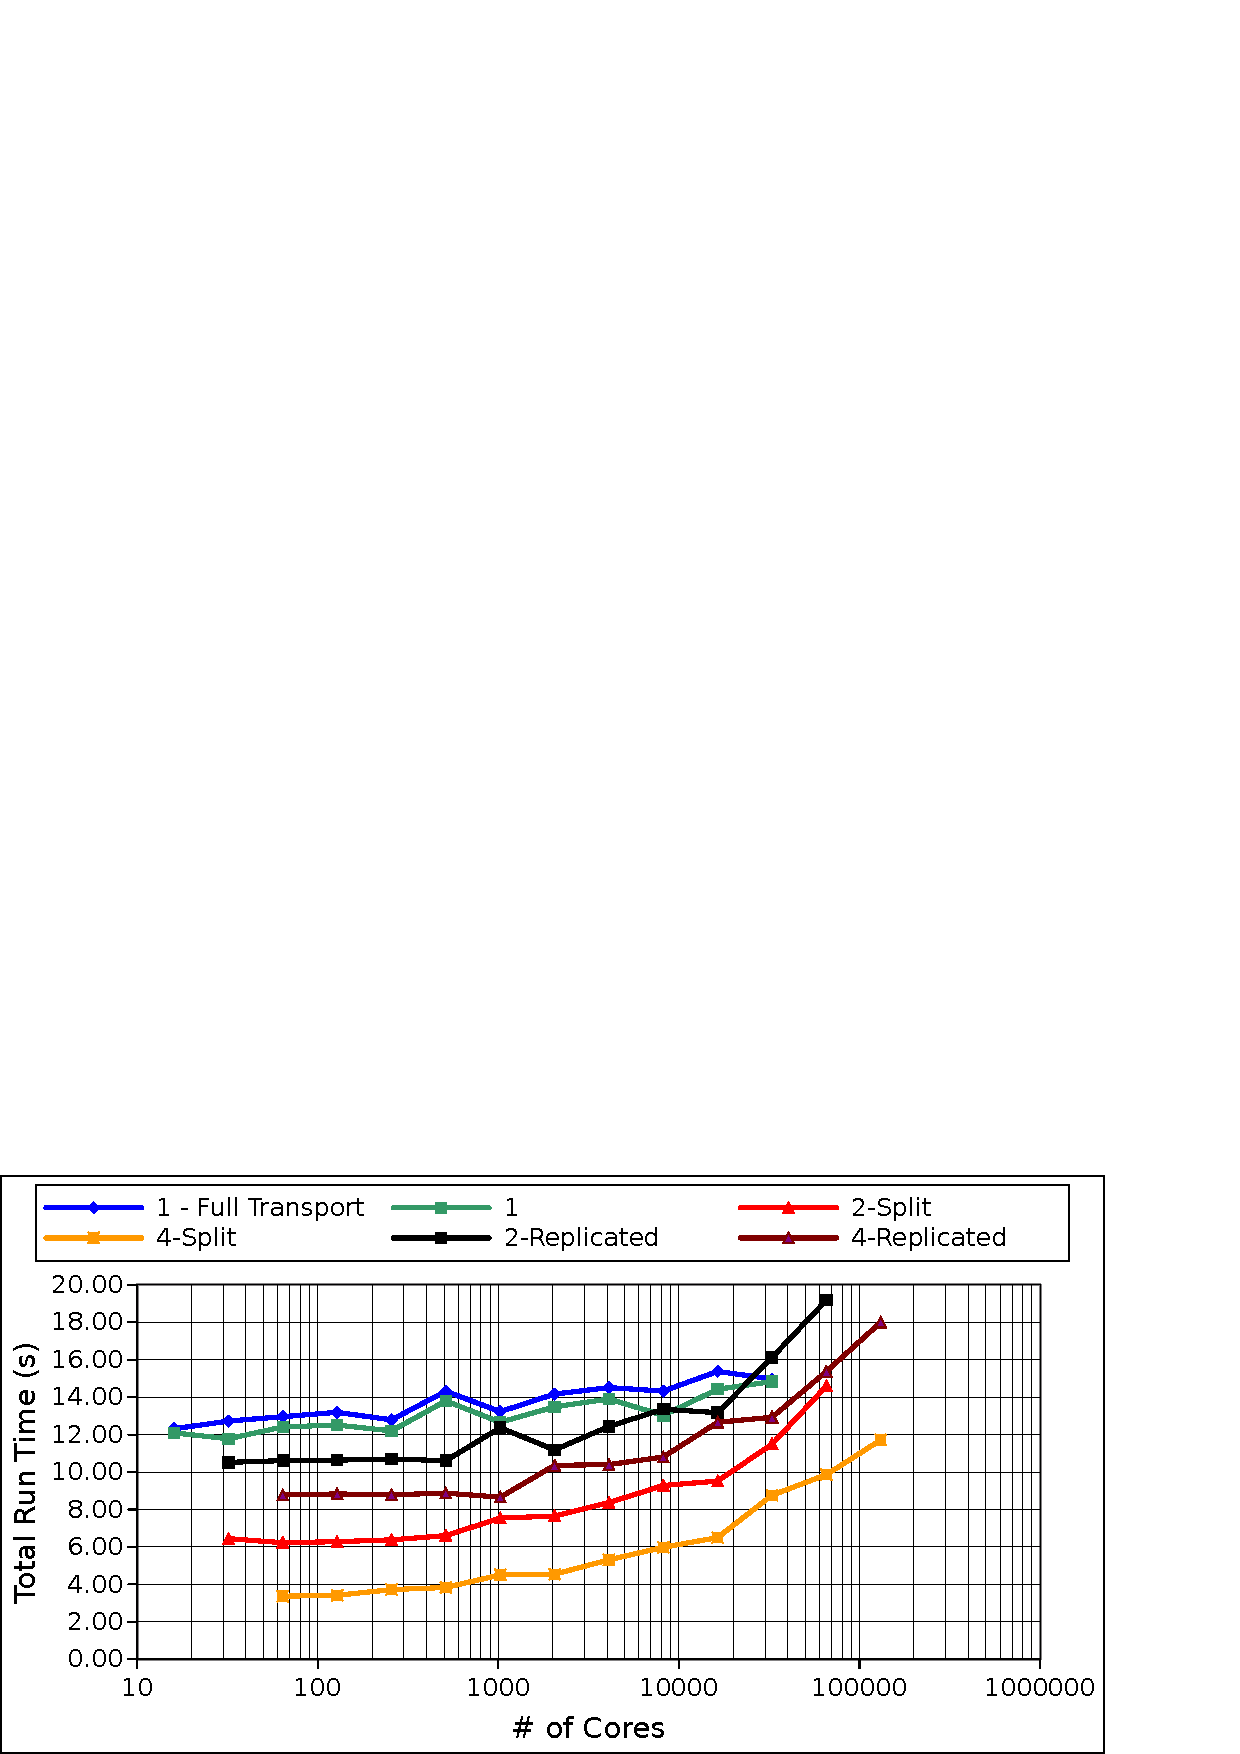
\includegraphics[width=6in]{chapters/parallel_mc/titan_weak_subdomain_ms_time.pdf}
  \end{center}
  \caption{\textbf{Weak scaling total wall time with multiple sets and
      subdomain Monte Carlo.} \textit{The addition of the set tally
      reduction is significant with cost of the reduction observed as
      core count grows.}}
  \label{fig:titan_weak_subdomain_ms_time}
\end{figure}

\begin{figure}[t!]
  \begin{center}
    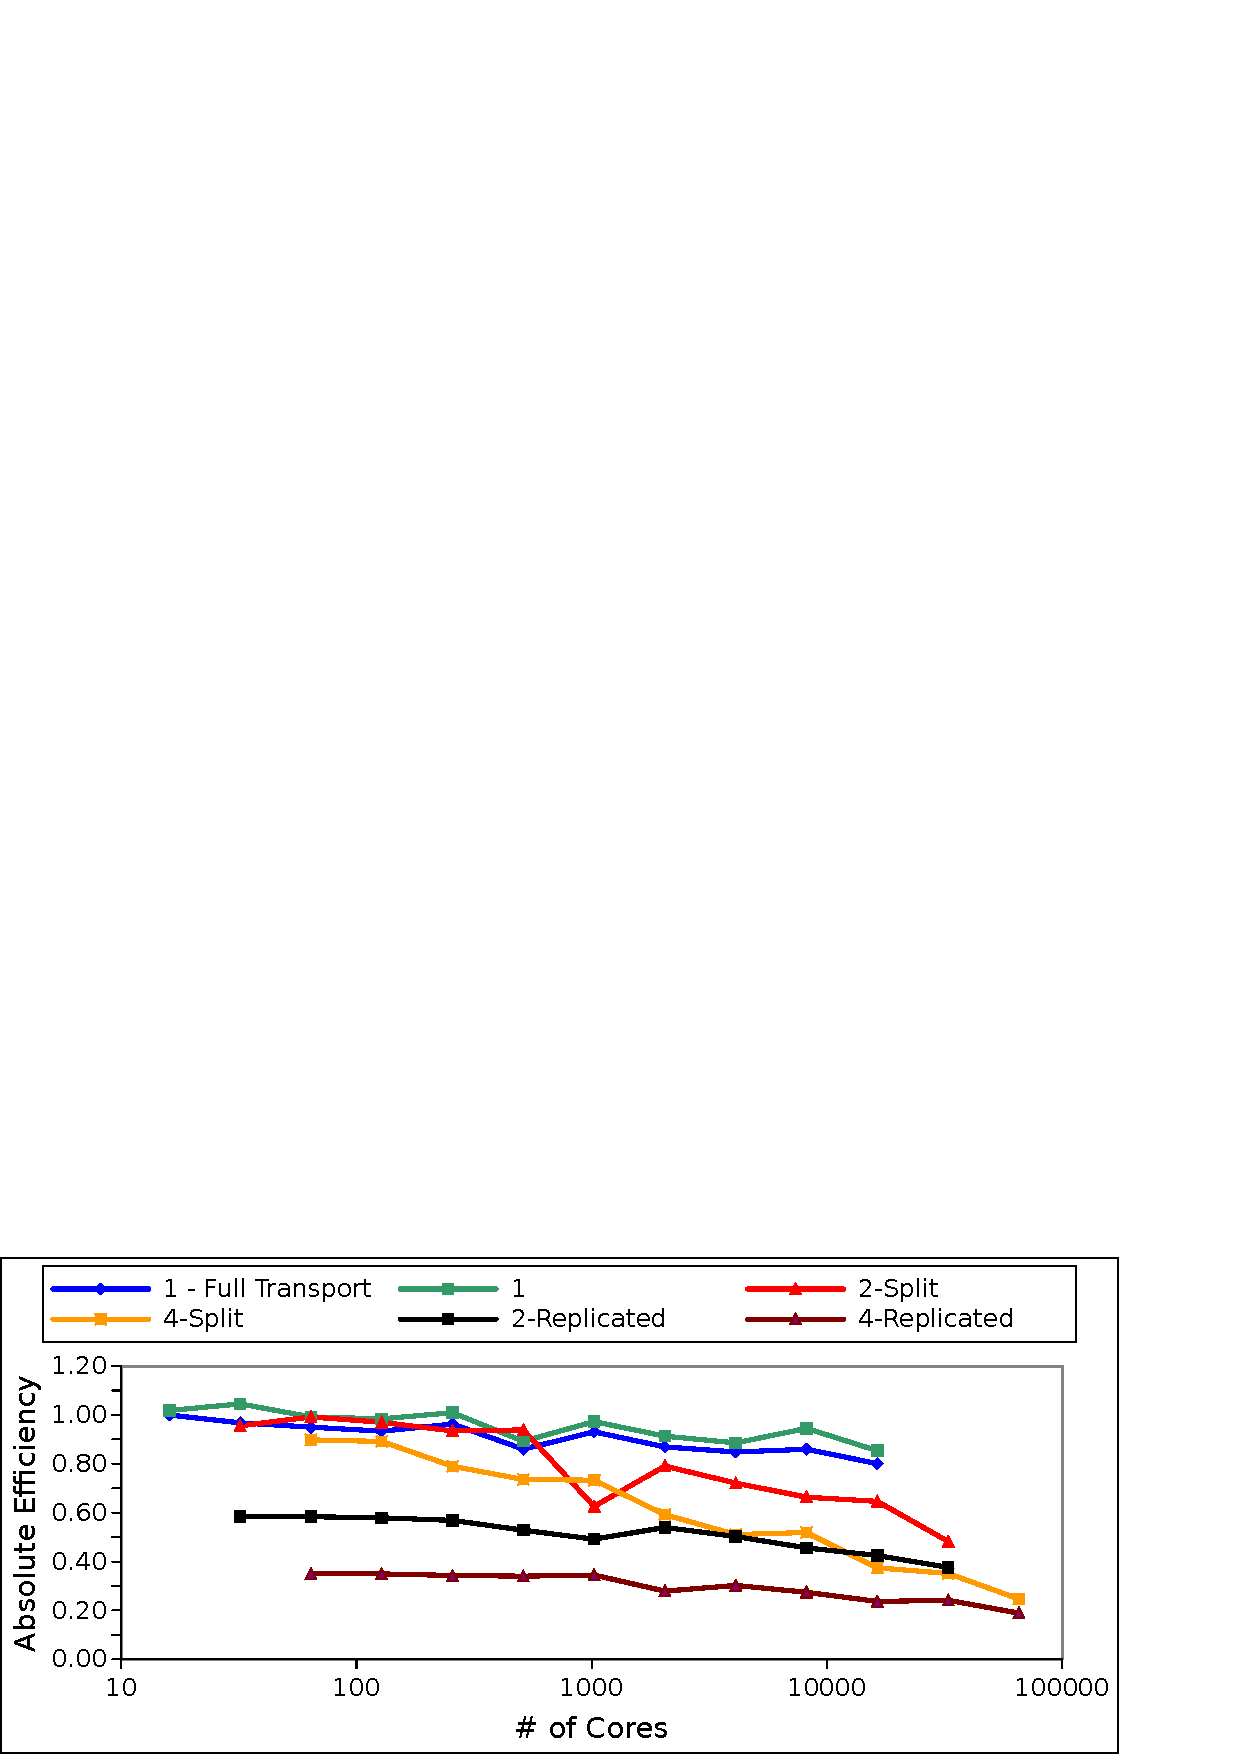
\includegraphics[width=6in]{chapters/parallel_mc/titan_weak_subdomain_ms.pdf}
  \end{center}
  \caption{\textbf{Weak scaling absolute efficiency for with multiple
      sets and subdomain Monte Carlo.} \textit{Weak scaling
      efficiencies are not improved at large core counts when multiple
      sets are added.}}
  \label{fig:titan_weak_subdomain_ms}
\end{figure}
